{\fontsize{12pt}{22pt} \textbf{Parametric Tests}\par}

\vspace{5mm}

A test is \textit{parametric} if its goal is to test parameters of a known/unknown distribution.

\vspace{5mm}

Procedure:

1) find the test to perform

2) find the right estimator to use

3) deduce the reject region

4) compute the test statistic

5) retrieve quantiles of known distributions

\vspace{5mm}

Example 1 \textbf{(\textbf{Gaussian-test})}: 

\vspace{5mm}

(\textit{inspired from example in Saporta p.325})

\vspace{5mm}

$X_1,...,X_n~(iid)\sim \mathbb{P_\theta}$

\vspace{5mm}

We want to analyze the mean. $m=a$?

\vspace{5mm}

1) find the test to perform

\vspace{5mm}

$
\left\{
    \begin{array}{ll}
        \mathcal{H}_0: m=a \\
        \mathcal{H}_1: m>a \\
    \end{array}
\right.
$

\vspace{5mm}

2) find the right estimator to use

\vspace{5mm}

Since we are testing the mean, we choose the empirical mean as \textbf{estimator} $\widehat{\theta}=\frac{1}{n}\sum{X_i}$

\vspace{5mm}

3) deduce the reject region

\vspace{5mm}

We fix $k$ for a rejection level $\alpha$. The rejection region is:

$Z=\{\widehat{\theta} \ge k\}$

\vspace{5mm}

We look for $k$ defined as such:

$\mathbb{P}_{\theta \in \Theta_0}(\widehat{\theta} \ge k)=\alpha$ => under $\mathcal{H}_0$, we reject the hypothesis when our estimator $\widehat{\theta}$ is above $k$

\textit{Intuitively, we want to keep our hypothesis if it's verified in most of the cases => under our hypothesis, there is a low probability that we are in the rejection region.}

\textit{Thus, if in real life we have a result that makes the hypothesis unverified, we reject the hypothesis. However, we have a risk of $\alpha$ that our hypothesis was correct and that we ended up in the rejection region by mistake.}

\vspace{5mm}

4) compute the test statistic

\vspace{5mm}

We center and reduce the estimator in order to get the Gaussian law and thus end up with known quantiles:

$\mathbb{P}_{\theta = a}(T \ge \frac{\sqrt{n} (k-a)}{\sqrt{\sigma^2}})=\alpha$ with $T \sim_{n \to \infty} \mathcal{N}(0,1)$

$T$ is the test statistic (\textcolor{red}{a test statistic is a random variable for which we know the law under $\mathcal{H}_0$})

\vspace{5mm}

5) retrieve quantiles of known distributions

\vspace{5mm}

Finally, $\frac{\sqrt{n} (k-a)}{\sqrt{\sigma^2}}=q_\alpha$ => we can find $k$ telling us when rejecting $\mathcal{H}_0$

\vspace{5mm}

\textcolor{gray}{Why not looking at the average directly?}

=> the average can be influenced by the outliers and thus doesn't take into consideration extreme events.

\vspace{5mm}

\textcolor{gray}{How about the median?}

=> the median doesn't take into account the distribution / tendency of the values.

\vspace{5mm}

$\alpha$ is also called the p-value. The lower the p-value is, the less error we make in rejecting our hypothesis so the more significant the rejection is.

\textcolor{red}{p-value is the lowest error probability we want to make when rejecting our hypothesis.}

\vspace{5mm}

When performing OLS, our hypothesis is $\theta_{x1}=0$ so we don't reject it if the pvalue column is higher than our threshold. In the below OLS result, pvalues are displayed in column $P>|t|$. All variables are significant.

\begin{center}
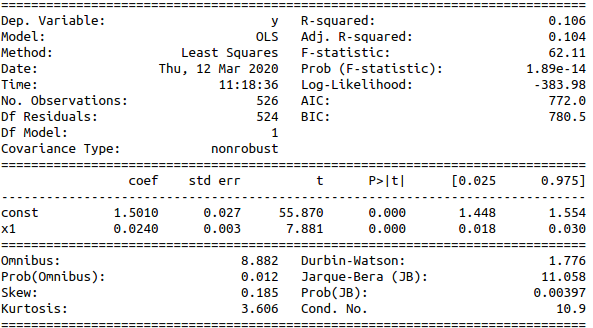
\includegraphics[scale=0.5]{OLS_pvalue.png}
\end{center}

Example 2 (\textbf{T-test}):  when the variance is not known.

\vspace{5mm}

Say we want to test whether a coefficient is zero:

1) find the test to perform

\vspace{5mm}

$
\left\{
    \begin{array}{ll}
        \mathcal{H}_0: \theta_j=0 \\
        \mathcal{H}_1: \theta_j \neq 0 \\
    \end{array}
\right.
$

\vspace{5mm}

2) find the right estimator to use

\vspace{5mm}

$\widehat{\theta_j} = (X^TX)^{-1}X^TY$

\vspace{5mm}

3) deduce the reject region

\vspace{5mm}

$Z=\{k_1 \leq \widehat{\theta_j} \leq k_2\}$

\vspace{5mm}

4) compute the test statistic

\vspace{5mm}

$T_j = \frac{\widehat{\theta_j}-\theta_j}{\sigma_{\theta_j}} = \frac{\widehat{\theta_j}}{\sigma_{\theta_j}}  \sim \mathcal{N}(0,1)$ with $\sigma_{\theta_j} = \sigma \sqrt{(X^TX)^{-1}}$ (recall that $\sigma = \sigma_{\epsilon}$)

\vspace{5mm}

Since we don't know $\sigma$, we can use the Cochrane theorem to remove this value:

$T_j = \frac{ \frac{\widehat{\theta_j}}{\sigma \sqrt{(X^TX)^{-1}}} \sim \mathcal{N}(0,1)}{\sqrt{\frac{\widehat{\sigma}^2 (n-p-1)}{\sigma^2} \sim \mathcal{X}_{n-p-1}}} \sim \mathcal{T}(n-p-1)$ with $\widehat{\sigma}^2 = \frac{1}{n-p-1} \Sigma \epsilon ^2$

$ T_j = \frac{\widehat{\theta_j}}{\Sigma \epsilon ^2 \sqrt{(X^TX)^{-1}}}$

\vspace{5mm}

5) retrieve quantiles of known distributions

\vspace{5mm}

Finally,


$\mathcal{P}_{\theta_j=0}(\frac{k_1}{\Sigma \epsilon ^2 \sqrt{(X^TX)^{-1}}} \leq T_j \leq \frac{k_2}{\Sigma \epsilon ^2 \sqrt{(X^TX)^{-1}}}) = \alpha$

Thus, $\frac{k_1}{\Sigma \epsilon ^2 \sqrt{(X^TX)^{-1}}} = t_{\frac{\alpha}{2}}$ (same for $k_2$)

\vspace{5mm}

Example 3 (\textbf{T-test} with forward selection):

\vspace{5mm}

Concept: 

Regress all variables one by one on the most significant variable's residual, remove the most significant variable after each full round

\vspace{20mm}

\begin{algorithm}
\caption{Forward selection}
\begin{algorithmic}
\State $sel \_ variables \leftarrow \emptyset$
\For{$i=1$ to $nb \_variables$}
\State $resid \_mem \leftarrow \emptyset$
\State $T \_stats \leftarrow \emptyset$
\For{$j=1$ to $rem \_ variables$}
\State $Y = X_j\theta$
\State $resid \_mem \leftarrow resid \_mem + \{res\}$ // adding residuals from previous regression
\State $T \_ stats \leftarrow T \_stats + \{T_j\}$ // $T_j$ is computed as seen in example 2
\EndFor
\State $k \leftarrow argmax(T \_ stats)$
\State $Y = resid \_ mem (k)$
\State $rem \_ variable \leftarrow rem \_ variable - \{k\}$
\State $sel \_ variables \leftarrow sel \_ variables + \{k\}$
\EndFor
\end{algorithmic}
\end{algorithm}

\begin{center}
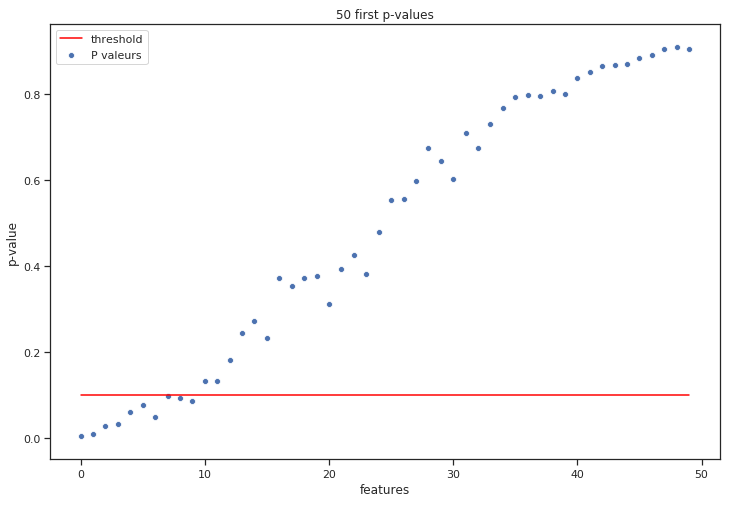
\includegraphics[scale=0.5]{forward_sel_pval.png}
\end{center}

(x-axis is the order in which we selected variables; see notebook \textit{ACP\_ForwardSelection\_Ridge\_Lasso.ipynb})

We can then select only the most significant variables based on p-values on variables from list $sel \_ variables$

\textit{Note}: since $pval = 2*(1-cdf(T)) = 2*\frac{1-(1-\alpha)}{2}$, choosing the biggest T-stat is equivalent to choose the smallest p-value

\vspace{5mm}

Example 4 (\textbf{F-test}):

\vspace{5mm}

When several variables are correlated (often the case in practice), the student test is not efficient enough since it does not take the correlation into account. F-test allows to test \textbf{global} significativity.

Let's say we have 4 variables and we want to check the significativity of 2 of them.

\vspace{5mm}

$
\left\{
    \begin{array}{ll}
        \mathcal{H}_0: \theta_1 = \theta_2 = 0\\
        \mathcal{H}_1: \theta_1, \theta_2 \neq 0 \\
    \end{array}
\right.
$

\vspace{5mm}

$SSR = sum~squared~residuals = \Sigma (\widehat{y_i} - y_i)^2$

\vspace{5mm}

$F = \frac{(SSR_C - SSR_{NC})/(p_{NC} - p_C)}{(SSR_{NC})/(n-p_{NC})} \sim \mathcal{F}(p_{NC} - p_C, n-p_{NC})$

\vspace{5mm}

NC: not constraint model

C: constraint model

\vspace{5mm}

Method:

- OLS on not constraint model => computation of $SSR_{NC}$

- OLS  on constraint model => computation of $SSR_{C}$

- Computation of the Fisher stat => computation of p-value (using complementary cumulative distribution function as above)

\lstset{language=Python}
\lstset{frame=lines}
\lstset{caption={F-test}}
\lstset{label={lst:code_direct}}
\lstset{basicstyle=\footnotesize}
\begin{lstlisting}

# Non constraint model
X0=np.column_stack((educ, exper, tenure, const))
model=sm.OLS(y,X0)
results = model.fit()
u=results.resid
SSR0=u.T@u

# Constraint model
X=np.column_stack((const, educ, tenure))
model=sm.OLS(y,X)
results = model.fit()
u=results.resid
SSR1=u.T@u

# Computation of Fisher stat
n=np.shape(X0)[0]
F=((SSR1-SSR0)/1)/(SSR0/(n-4))
f.sf(F,1,n-4) # p-value

\end{lstlisting}


\vspace{5mm}